\section{FESDModelv2 Results}

\subsection{Full Body Error Estimation}
\ref{sec:full_body}

The first and most general model that was developed was the full body model. The full body model was trained to give a single error label as an output given an image as an input. The results of the training process of the Full Body model can be seen in figure \ref{fig:full_body_training_results}.

The result of the training is rather disappointing. The testing showed that the model only performs well on the training data. The model does not generalise well to new data. The reason for this is that the model is overfitting. The model is overfitting because the model is too complex for the amount of data that is available. The model has 21.5 million trainable parameters. This is too many parameters for the amount of data that is available. The model is not able to learn the underlying patterns of the data, but rather memorises the training data. This is also shown in the training and testing loss. The training loss is decreasing, but the testing loss is increasing. This is a clear sign of overfitting.

\subsubsection{Confusion Matrix}

The confusion matrix of the full body model is shown in figure \ref{fig:full_body_confusion_matrix}. It can be seen that the model only predicts the error label $0$ - No Error. This is because the model is overfitting.

\begin{figure}
  \centering
  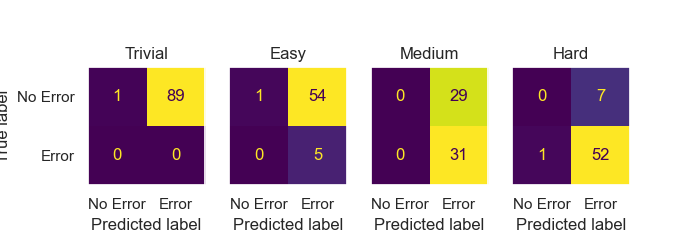
\includegraphics[width=0.8\textwidth]{figures/results/confusion/full.png}
  \caption[Full Body model confusion matrix]{The confusion matrix of the full body error estimation model.}
  \label{fig:full_body_confusion_matrix}
\end{figure}

\subsection{Half Body Error Estimation}
\label{sec:half_body}

The second model that was developed was the half body model. The half body model was trained to give two error labels as an output given an image as an input, one for the lower body and one for the upper body. The results of the training process of the Half Body model can be seen in figure \ref{fig:half_body_training_results}.


\subsubsection{Confusion Matrix}

The confusion matrix of the half body model is shown in figure \ref{fig:half_body_confusion_matrix}. It can be seen that contrary to the full body model the half body model variies the error label. 

\begin{figure}
  \centering
  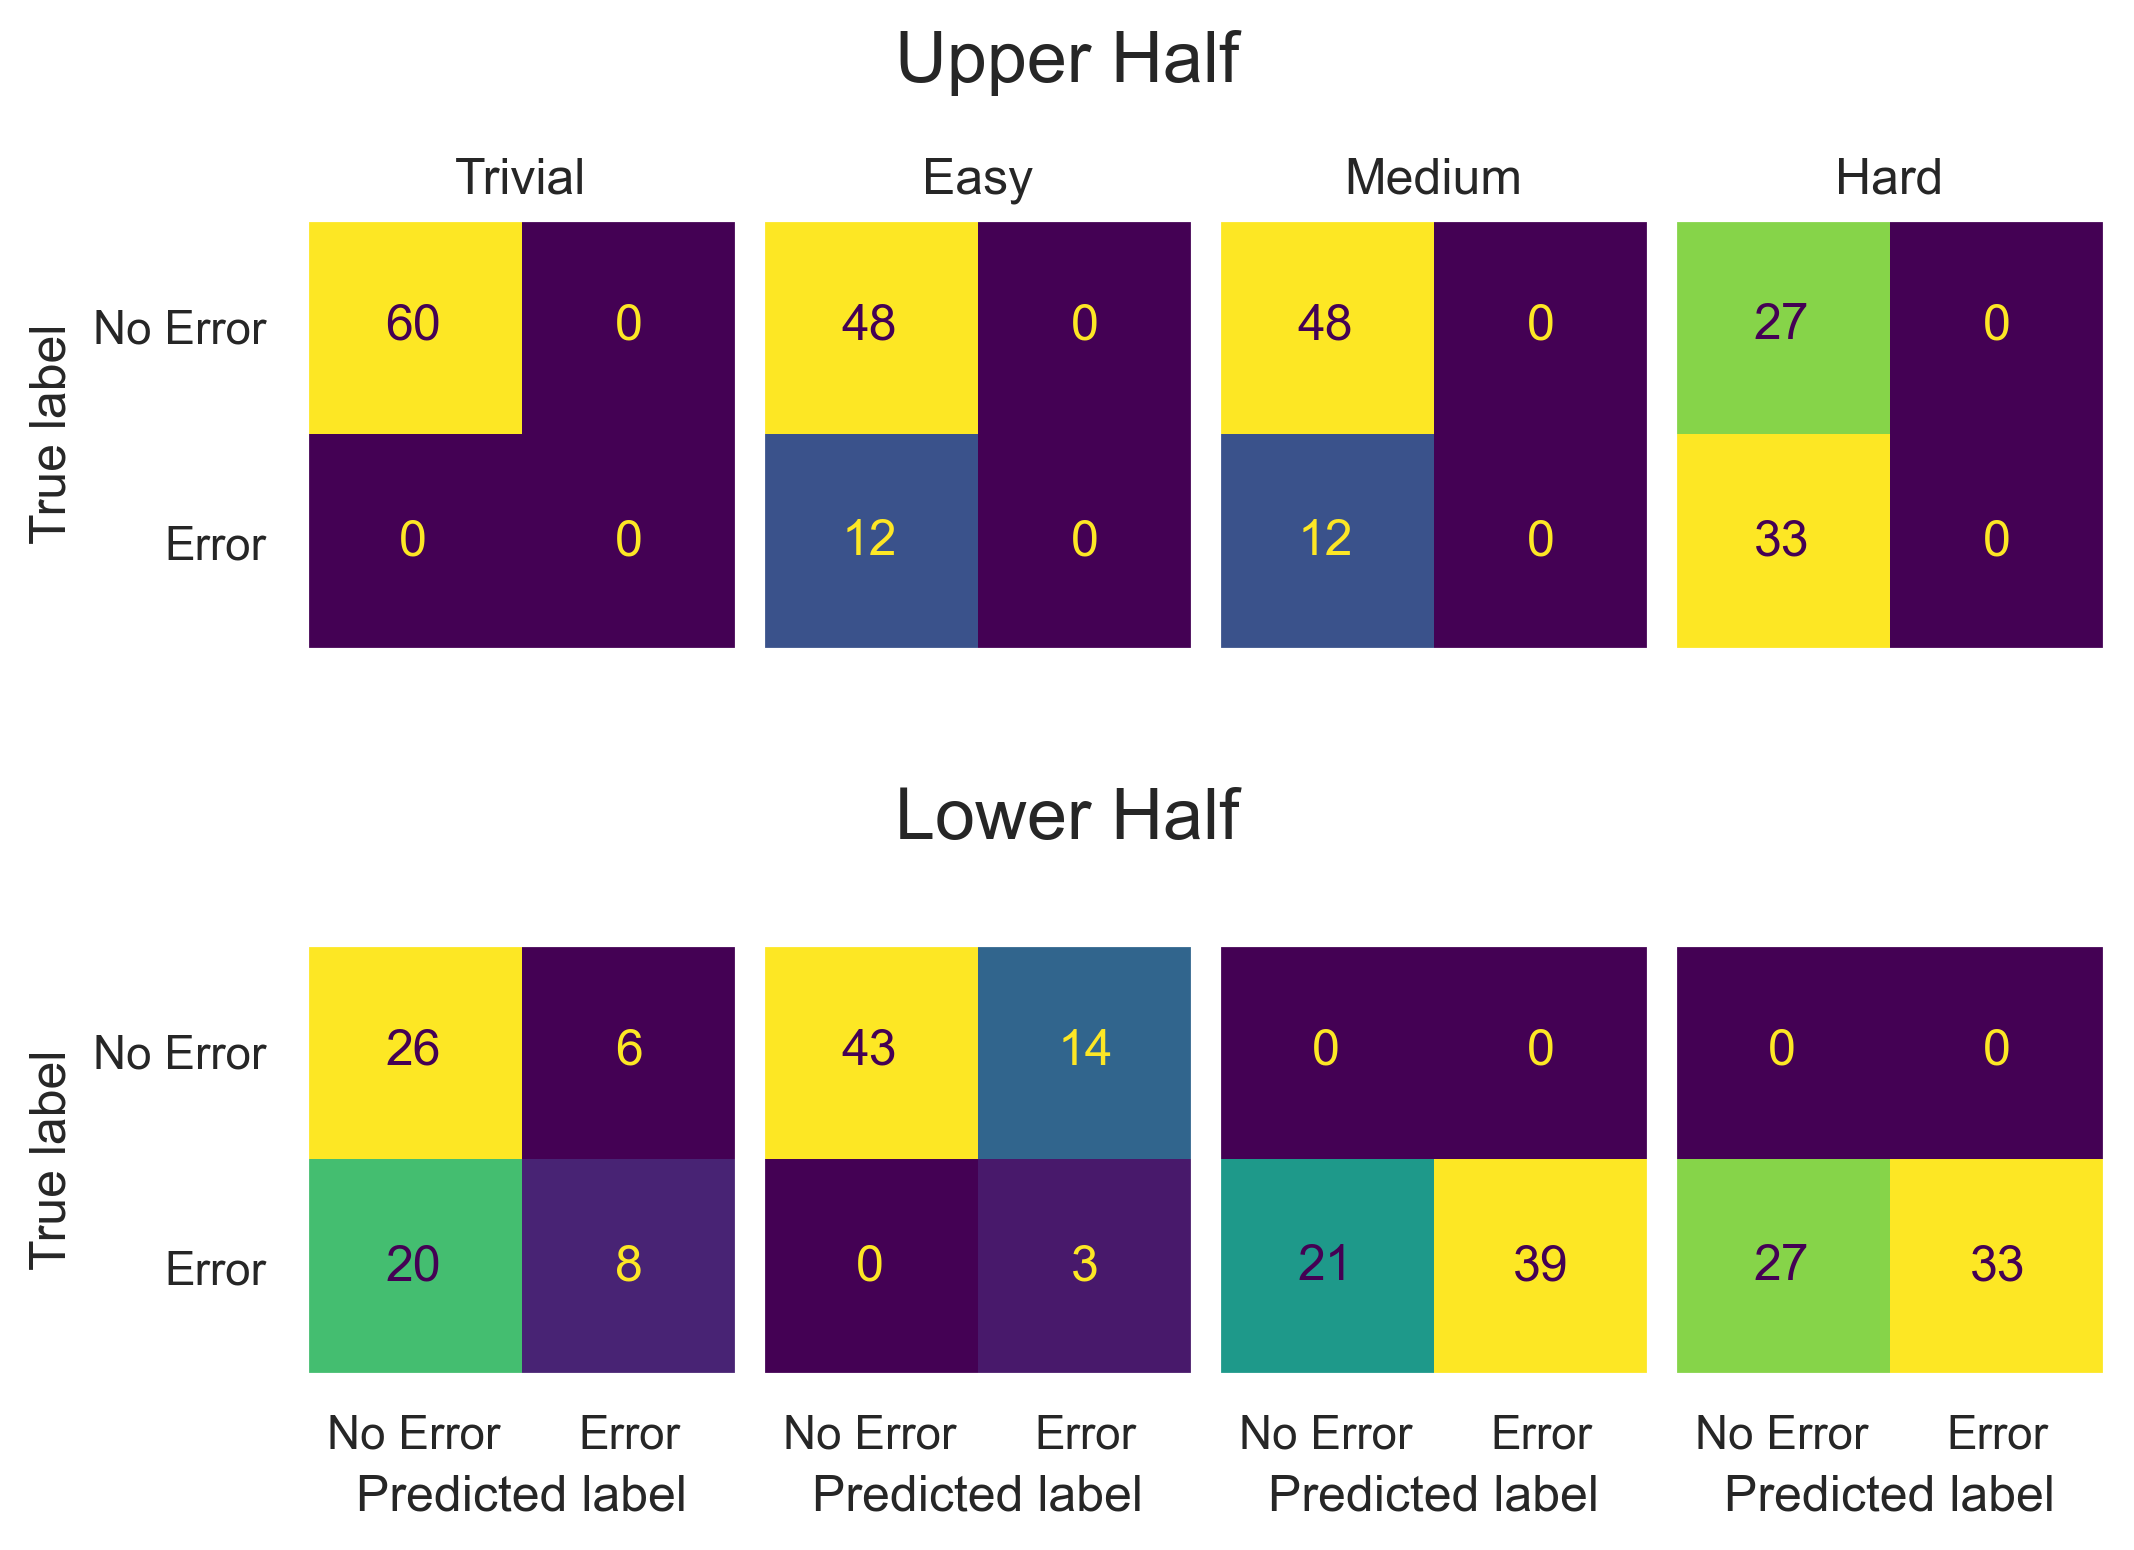
\includegraphics[width=0.8\textwidth]{figures/results/confusion/halves.png}
  \caption[Half Body model confusion matrix]{The confusion matrix of the half body model.}
  \label{fig:half_body_confusion_matrix}
\end{figure}

\subsection{Limb Error Estimation}
\label{sec:limb_error_estimation}

The results for the limb error estimation are the same as for the full body error estimation. The model is overfitting and therefore only predicts the error label $0$ - No Error for most cases. The results of the training process of the Limb model can be seen in figure \ref{fig:limb_training_results}.


\subsubsection{Confusion Matrix}

The confusion matrix of the limb model is shown in figure \ref{fig:limb_confusion_matrix}. It can be seen that the model only predicts the error label "No Error" or "Error" for most joints without variation. This is because the model is overfitting.

\begin{figure}
  \centering
  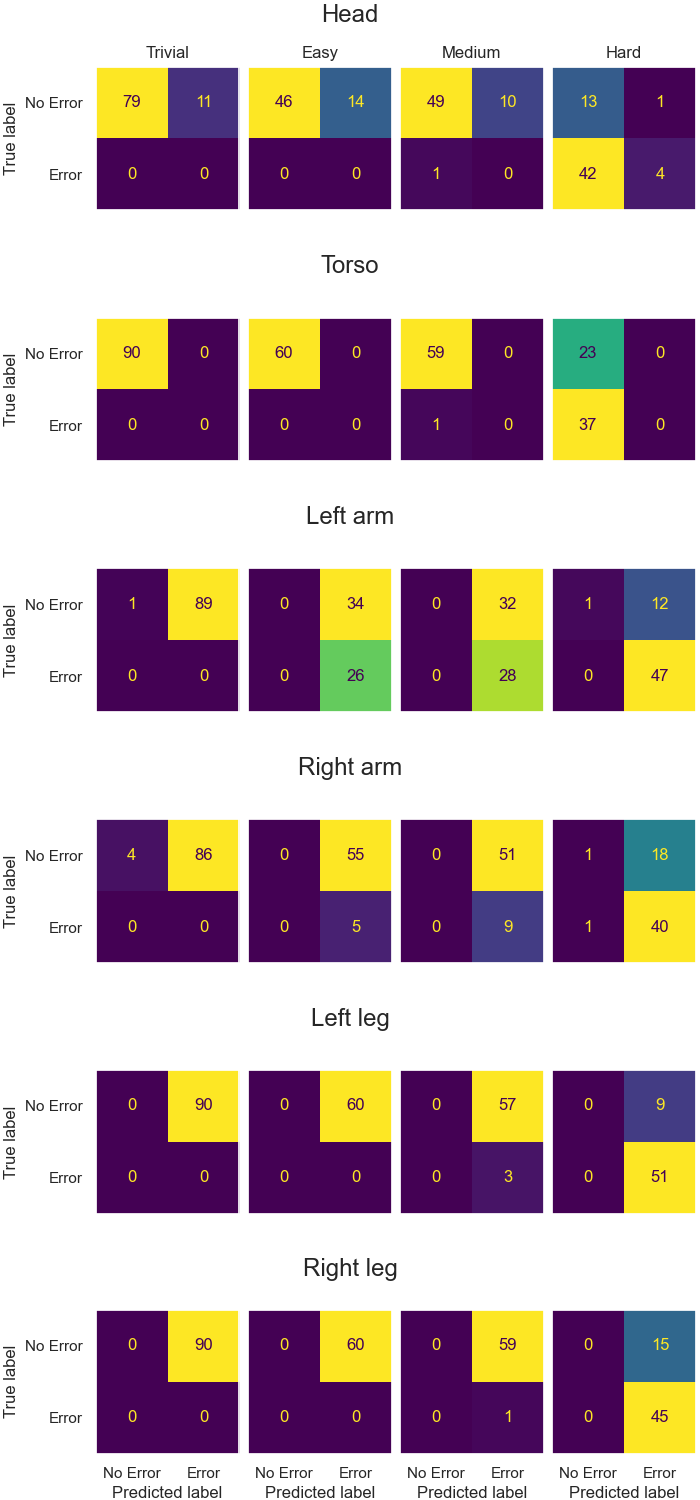
\includegraphics[width=\textwidth]{figures/results/confusion/limbs.png}
  \caption[Limb model confusion matrix]{The confusion matrix of the limb model.}
  \label{fig:limb_confusion_matrix}
\end{figure}

\subsection{Joint Error Estimation}
\label{sec:joint_error_estimation}

The results for the joint error estimation are the same as for the full-body error estimation. The model is overfitting and therefore only predicts the error label $0$ - No Error for most joints. The results of the training process of the Joint model can be seen in figure \ref{fig:Joint_training_results}.

\subsubsection{Confusion Matrix}

The confusion matrix of the joint model is shown in figure \ref{fig:joint_confusion_matrix}(TODO: split that graph, its huge). It can be seen that the model only predicts the error label $0$ - No Error for most joints. This is because the model is overfitting.

\begin{figure}
  \centering
  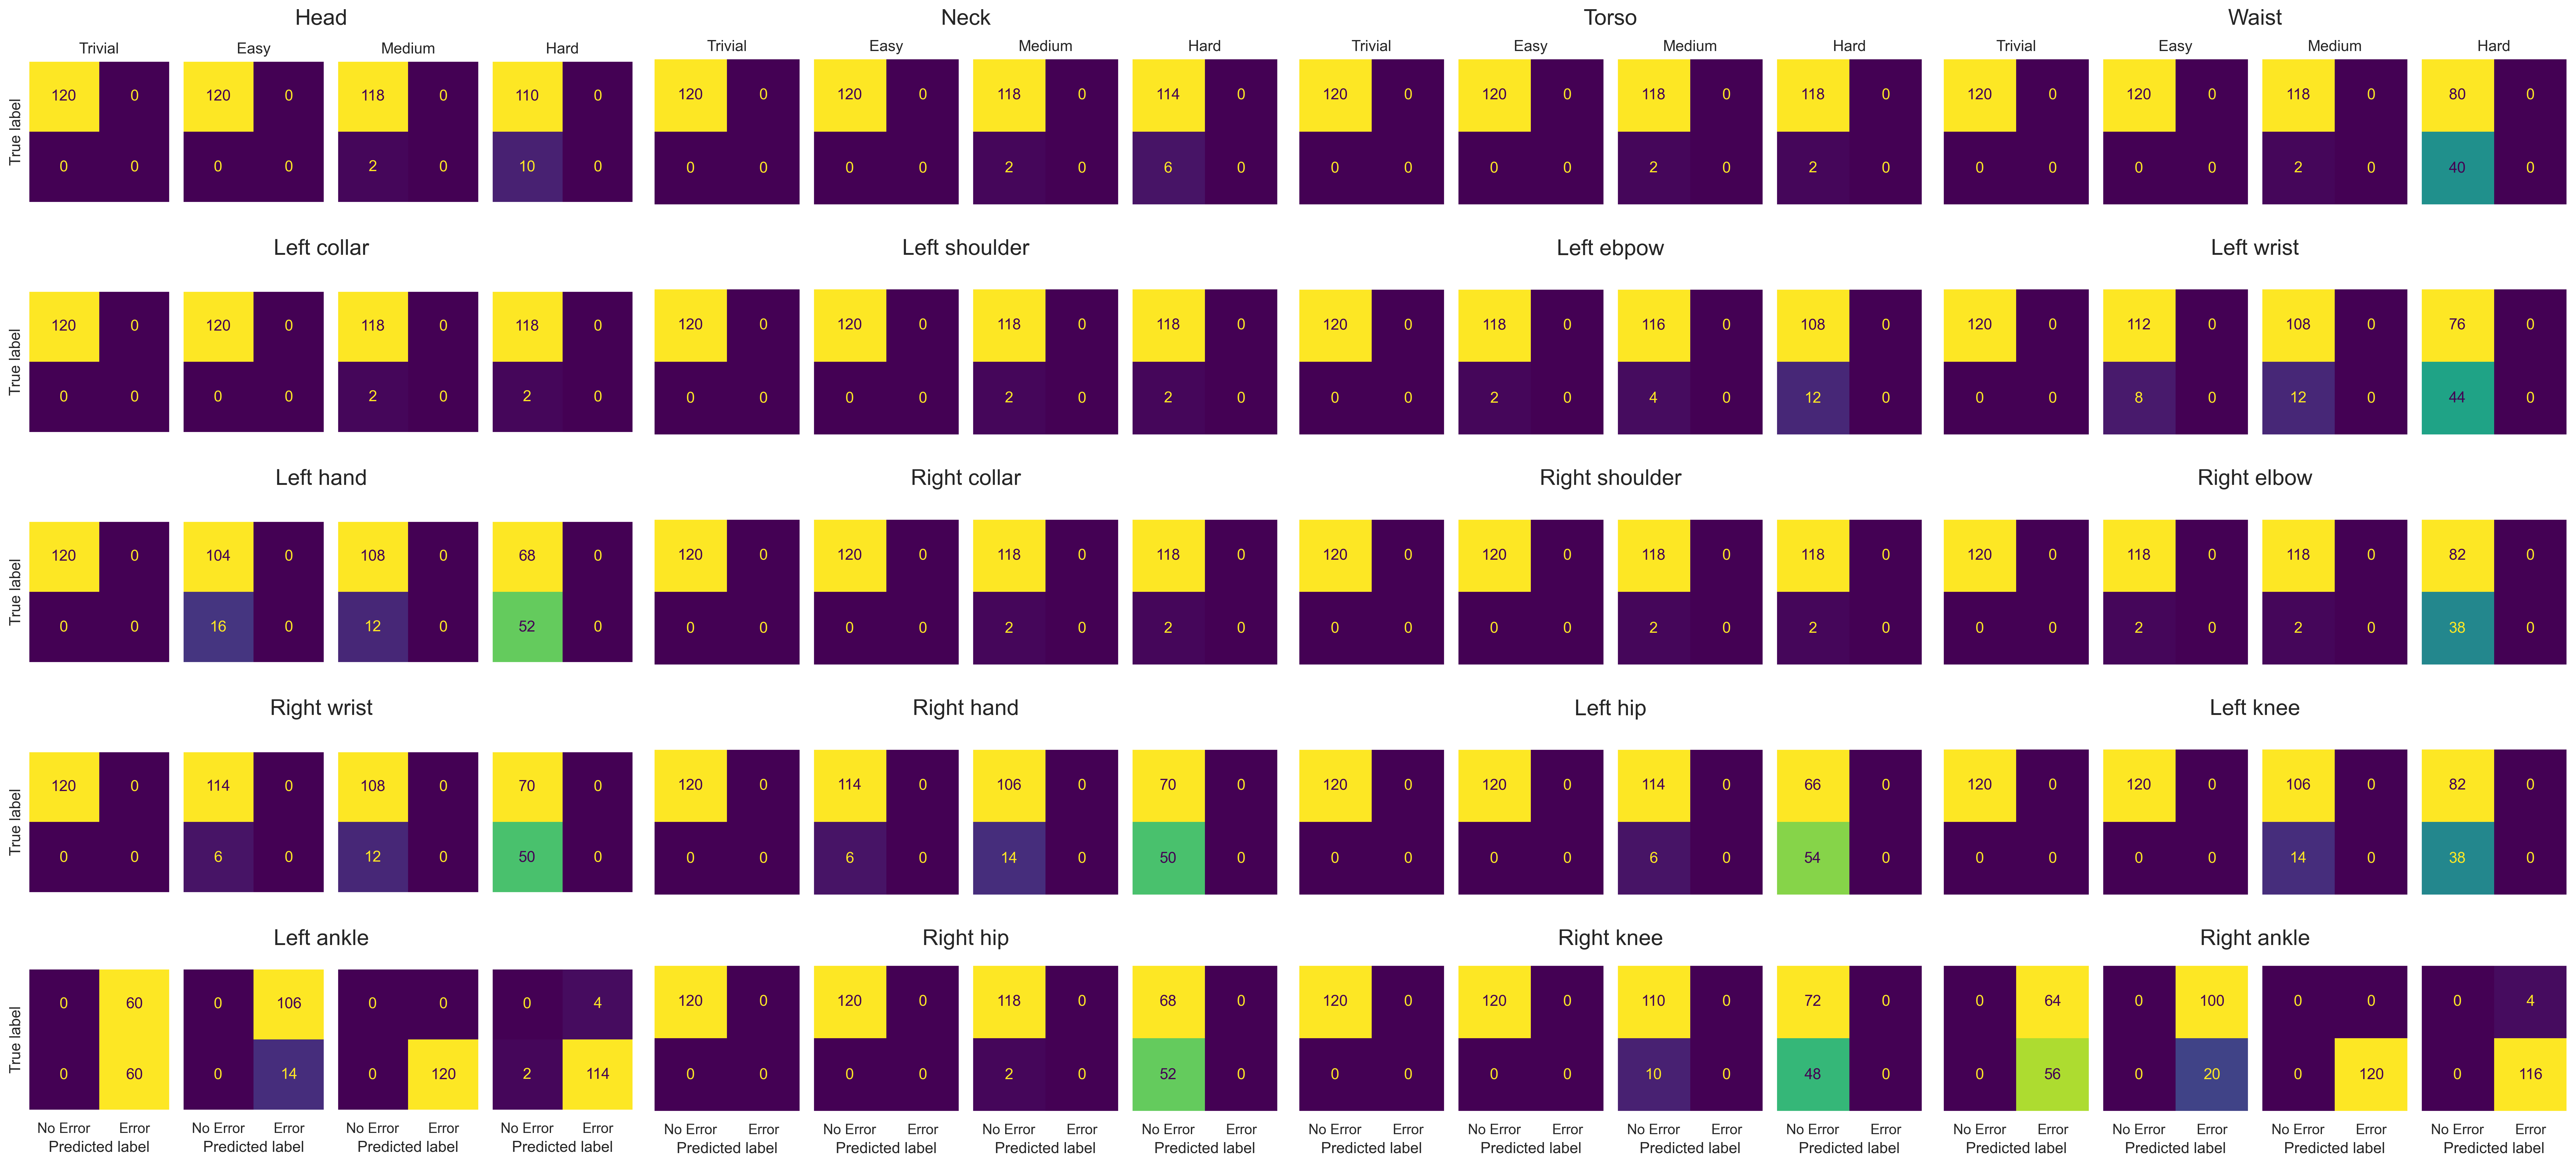
\includegraphics[width=\textwidth]{figures/results/confusion/joints.png}
  \caption[Joint model confusion matrix]{The confusion matrix of the joint model.}
  \label{fig:joint_confusion_matrix}
\end{figure}